\chapter{Experiment}

Experimentom v našej práci je určovanie hĺbky pamäte a vyhodnotenie vplyvu rôznych
hyper parametrov a typov kontextov na hĺbku pamäte rekurentných SOM.
Cieľom nášho experimentu je aj nájdenie 
optimálnej kombinácie parametrov pre všetky typy porovnávaných sietí a ich vzájomné porovnanie.

\section{Výber konkrétnych trénovacích množín pre experiment}
Trénovacie množiny sme sa snažili zvoliť
takým spôsobom aby sme na nich vedeli otestovať rôzne vlastnosti rekurentných sietí.

Pre náš experiment sme vybrali 3 trénovacie množiny.
Hlavnou trénovaciou množinou, ktorú používame v našom experimente je náhodne generovaná 
sekvencia dlhá 1000 znakov, ktorá pozostáva z písmen $abcd$.
Táto sekvencia obsahuje dostatočné množstvo regularít a malé množstvo unikátnych znakov a teda
aj siete s relatívne malým počtom neurónov sa na nej vedia dobre natrénovať.
Používame ju pri hľadaní optimálných parametrov pre jednotlivé typy sietí.

Ako druhú trénovaciu množinu sme zvolili sekvenciu dlhú 1000 znakov, pričom znaky sú generované
špeciálnym pravdepodobnostným stavovým automatom (Reberov automat). Automat generuje znaky z množiny znakov $ptvxse$.
Táto sekvencia je pre SOMky ťažšia na naučenie a používame ju na overenie toho, či sú siete schopné natrénovať sa aj
na zložitejších nenáhodných sekvenciách. Pri SRN je použitie tejto trénovacej množiny zaujímavejšie,
vďaka vlastnostiam, ktoré SRN má.

Tretí dataset je úryvok z korpusu anglického textu.
Keďže ide o reálny zmysluplný text, nie je to úplne náhodná postupnosť znakov, ale obsahuje určité vzory a opakovania, ktoré by siete mohli vedieť zachytiť
vo svojej vnútorenej reprezentácii.
Tento dataset používame čisto iba na overenie, či 
sú SOMky schopné zachytiť vzory aj v prirodzenom jazyku a teda či sú použiteľné aj pre 
reálne dáta.

\section{Hľadanie optimálnych parametrov sietí}
Na to aby sme mohli porovnať hĺbku pamäte rôznych typov sietí museli sme najskôr
nájsť kombináciu parametrov pri ktorých daný typ siete dosahuje najnižšiu kvantizačnú chybu a 
najvyššie hodnoty pamäťových hĺbok. 

Pri trénovaní samoorganizujúcich sa máp môžeme meniť a optimalizovať veľké množstvo parametrov. 

Ako prvé sme museli správne nastaviť veľkosť okolia víťazného neurónu.
Veľkosť okolia by nemala byť počas trénovania konštantná, ale mala by sa postupne zmenšovať.
Vo fáze doľaďovania by mala byť čo najmenšia.
Excitáciu neurónu v určitom kroku trénovania určuje excitačná funkcia. Zvolili sme spojitú
excitačnú funkciu so spojitým gausovským okolím. 
\begin{equation}
    N(i^{*}, i) = \exp^{- \frac{d^{2}_{E}(i^{*}, i)}{\lambda^{2}(t)}}
\end{equation}
Najvyššiu hodnotu má excitačná funkcia pre víťazný neurón, hodnota excitačnej funkcie pre ostatné 
neuróny v sieti závisí od ich euklidovskej vzdialenosti v mriežke neurónov od ich víťaza. Veľmi vzdialené neuróny 
majú takmer nulovú excitáciu a updatujú svoje váhy minimálne.
Dôležitý je parameter $\lambda$, ktorým znižujem veľkosť okolia postupne v jednotlivých epochách.
Najlepšie výsledky (najnižšie hodnoty kvantizačnej chyby) sme dosiahli pri použití nasledujúceho vzťahu pre výpočet hodnoty tohto parametra
v jednotlivých epochách:
\begin{equation}
    \lambda{(t)} = \lambda_{i} \cdot (\lambda_{f} /\ \lambda_{i})^{t /\ t_{max}}
\end{equation}
Kde $\lambda_{f}$ je konštanta, ktorá určuje rýchlosť klesania. 
$\lambda_{i}$ je polovica maximálnej vzdialenosti dvoch neurónov v mape, resp. 
vzdialenosť dvoch neurónov na koncoch diagonály mriežky neurónov.
$t$ je číslo aktuálnej epochy trénovania. Parametrer $t_{max}$ je celkový počet 
epôch trénovania.

% rychlost ucenia
Rovnako ako okolie aj rýchlosť učenia siete by mala počas
procesu trénovania postupne klesať. Na začiatku chceme aby sa váhy menili čo najviac
a ku koncu učenia chceme aby sa doľadovali iba detaily.
Máme na výber 2 možnosti. Postupné znižovanie rýchlosti učenia v rámci jednej epochy, alebo 
postupné znižovanie rýchlosti učenia v jednotlivých epochách, pričom počas každej epochy
je rýchlosť učenia konštantná. 
V naších experimentoch sme dosiahli lepšie výsledky postupním 
znižovaním rýchlosti učenia v rámci jednej epochy. 
Hodnoty rýchlosti učenia máme z intervalu $<0, 1>$.

% veľkosť sliding window
Vhodnú veľkosť posuvného okna sme určili postupním zvyšovaním jeho veľkosti pokiaľ pamäťová hĺbka stúpala. 
Zaujímavosť, ktorú sme zistili počas experimentovania s veľkosťou pamäťového okna, bolo že 
ak zvolíme príliš veľké posuvné okno, výsledná pamäťová hĺbka môže byť skreslená.
Pri veľkom pamäťovom okne nám môžu neuróny, ktoré majú vo svojom pamäťovom okne uloženú iba 
jednu sekvenciu skreslovať výslednú pamäťovú hĺbku, pretože pamäťová hĺbka takýchto
neurónov je rovná veľkosti posuvného okna. Z tohto dôvodu nie je dobré nastaviť veľkosť pamäťového okna na 
príliš veľkú hodnotu, ale treba určiť optimálnu hodnotu.

% vyber rozmerov a pocet trenovacich epoch mapy
Rozmery mapy a počet trénovacích epôch sme zvolili na základe vlastností zvolenej trénovacej množiny. 
Tiež sme museli brať do úvahy aj časovú náročnosť trénovania sietí (najmä pri RecSOM).
Potrebovali sme aby sa sieť dokázala správne natrénovať na danej trénovacej množine a zároveň, aby nám experimenty dobehli v rozumnom čase.
Keďže SOMky sa dokážu natrénovať relatívne rýchlo, zvolili sme väčšie rozmery mapy (30x30) a o niečo nižší počet trénovacích epôch (10).
S touto kombináciou sme dosiahli nízke hodnoty kvantizačných chýb a dobré hodnoty pamäťových hĺbok.


\subsection{Parametre pre RecSOM}
Pri RecSOM kontext tvorí vektor aktivít neurónov z predchádzajúceho kroku.
Aktivita neurónu $y$ je určená vzťahom:

\begin{equation}
    y_{i} = \exp{(-d_{i})}
\end{equation}

Neobsahuje žiadny meniteľný parameter. Hodnota $d_{i}$ je súčet vzdialenosti vstupného vektora od váhového vektora a kontextového vektora od 
kontextového vektora. So zmenšujúcou sa vzdialenosťou excitácia neurónu rastie exponenciálne, čo 
znamená, že víťaz a susedné neuróny budú mať najvyššiu excitáciu a vzdialené neuróny budú mať malú excitáciu.
Výpočet kontextu pri RecSOM nevieme ovplyvnovať žiadnym parametrom.

Môžeme však meniť parameter $\alpha$, ktorý sa používa pri samotnom výpočte vzdialenosti
vstupu od váhového vektora a kontextu od vkontextového vektora. Tento parameter určuje váhu aktuálneho vstupu a váhu kontextu
vo výslednej vzdialenosti.
\begin{equation}
	d_i = (1 - \alpha) \cdot ||x(t) - w_i||^{2} + \alpha \cdot ||y(t-1) - c_i||^{2} \quad c \in R^{N}
\end{equation}
V našich experimentoch sme testovali všetky hodnoty parametra $\alpha$ z uzavretého intervalu
$<0, 1>$ s krokom $0.01$ (dokopy 100 experimentov).

\subsection{Výsledky pre RecSOM}

\begin{table}[h!]
    \centering
    \begin{tabular}{|c|c|} 
     \hline
     Parameter & Hodnota \\ 
     \hline\hline
     alpha & 0 - 1  (krok: 0.01) \\ 
     \hline
     size & 30x30  \\
     \hline
     počet epôch & 10  \\
     \hline
     veľkosť posuvného okna & 15  \\
     \hline
    \end{tabular}
    \caption{Trénovacie parametre RecSOM siete}
    \label{table:1}
    \end{table}

\begin{figure}[H]
    \centering
    \begin{subfigure}{.5\textwidth}
        \centering
        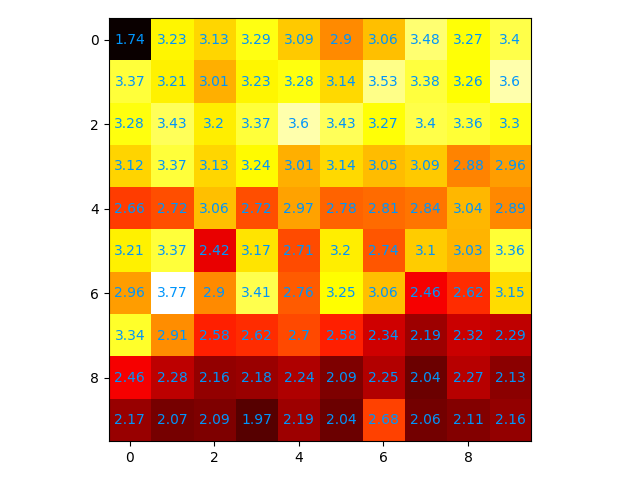
\includegraphics[width=\linewidth]{assets/recsom_memory_span}
        \caption{Recsom pamäťová hĺbka}
        \label{fig:sub1}
    \end{subfigure}%
    \begin{subfigure}{.5\textwidth}
        \centering
        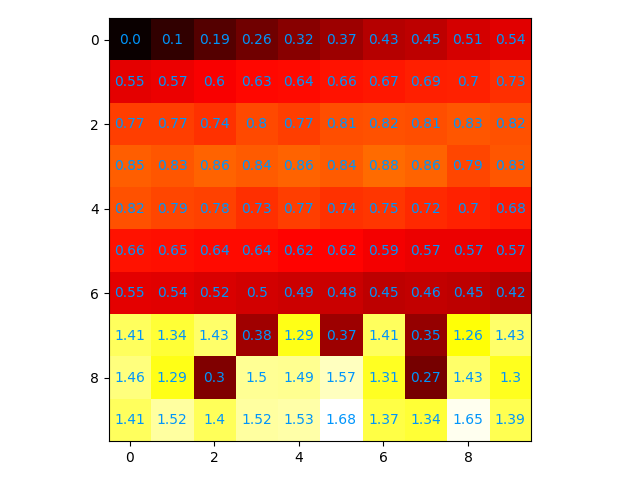
\includegraphics[width=\linewidth]{assets/recsom_quantization_errors}
        \caption{Recsom kvantizačné chyby}
        \label{fig:sub2}
    \end{subfigure}
    \caption{Heatmapy pre Recsom}
    \label{fig:test}
\end{figure}

\subsection{Analýza výsledkov RecSOM}

Hodnoty na x-ovej osy sú hodnoty $\alpha$  a na y-ovej 
osy sú hodnoty $(\alpha - 1)$. Čísla v jednotlivých políčkach sú pamäťové hĺbky 
pre danú kombináciu parametrov. Čím je farba políčka svetlejšia, tým je pamäťová hĺbka vyššia.
Čím je farba tmavšia, tým je hodnota nižšia.

Ak sú hodnoty oboch parametrov nulové, vtedy sieť dosahuje nízku hodnotu pamäťovej hĺbky pretože sa nedokáže správne natrénovať.


RecSOM dosiahla najvyššiu hodnotu pamäťovej hĺbky pri 
hodnote parametra $\alpha = 0.28$, resp. $(1 - \alpha) = 0.72$. To znamená, že
vo výpočte vzdialenosti má vzdialenosť od vstupu od váhového vektora váhu $0.72$
a vzdialenosť kontextového vektora od kontextových váh má váhu $0.28$.
Hodnota pamäťovej hĺbky, ktorú recSOM dosiahla je priemerná pričom samotné 
trénovanie bolo relatívne pomalé.
Všeobecne vo výsledkoch vidíme, že pamäťová hĺbka RecSOM nie je veľmi ovplyvňovaná hodnotou parametra $\alpha$ a rozdiely nie sú veľké. 
Je to pravdepodobne dané tým, že RecSOM má veľmi bohatý kontext, v ktorom sa uchováva veľké množstvo informácii (aktivita celej mapy). Skutočnosť že pamäťová hĺbka RecSOM nie
je signifikantne ovplyvnená váhou kontextu nám napovedá aj to, že informácie uchovávané v RecSOM kontexte nie sú relevantné pre hodnotu pamäťovej hĺbky a môžu mať skôr negatívny vplyb.

Pamäťovú hĺbku RecSOM ovplyvňuje váha aktuálneho vstupu
(hodnota $(\alpha - 1)$), čím je vyššia tým je väčšia pravdepodobnosť, že sieť dosiahne horšiu hodnotu pamäťovej hĺbky. Rovnako váha aktuálneho vstupu
ovplyvňuje aj samotné učenie siete, ako je možno vidieť na heatmape kvantizačných chýb. Pri hodnotách $>0.6$ sa už sieť v mnohých prípadoch nedokázala natrénovať správne.

 
\begin{figure}[H]
    \centering
    \begin{subfigure}{.5\textwidth}
        \centering
        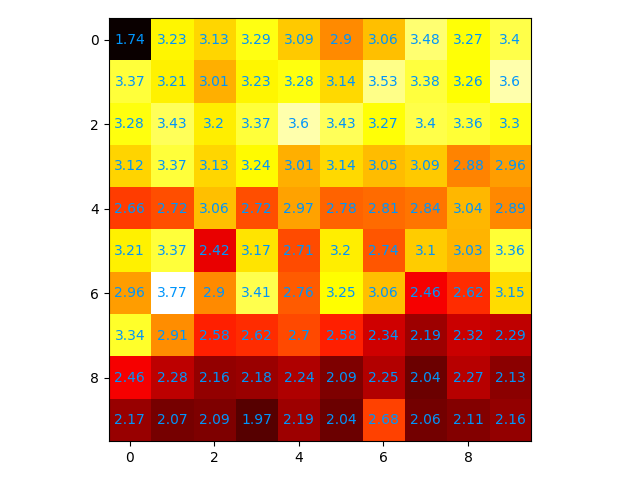
\includegraphics[width=\linewidth]{assets/recsom_memory_span}
        \caption{Recsom pamäťová hĺbka}
        \label{fig:sub1}
    \end{subfigure}%
    \begin{subfigure}{.5\textwidth}
        \centering
        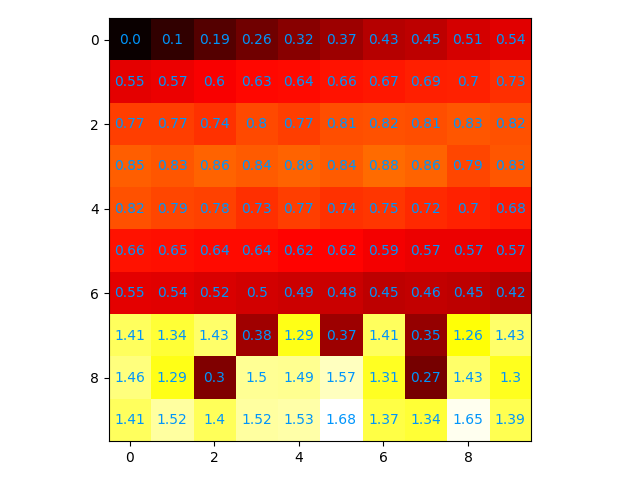
\includegraphics[width=\linewidth]{assets/recsom_quantization_errors}
        \caption{Recsom kvantizačné chyby}
        \label{fig:sub2}
    \end{subfigure}
    \caption{Heatmapy pre Recsom}
    \label{fig:test}
\end{figure}

% todo ukazka priebehu klesacujec kvantizacnej chyby pri najvhodnejsej kombinacii parametrov
% todo priemer kvantizacnych chyb s hodnotou najlepsieho parametra
% ukazka testov s najlepsimi parametrami

% výsledky experimentu

\subsection{Activity RecSOM}
Keďže pri obyčajnej verzii RecSOM nevieme ovplyvniť žiadnym parametrom výpočet kontextu. Preto sme sa 
rozhodli vytvoriť si modifikovanú verziu RecSOM. Rozdiel oproti pôvodnej verzii je v spôsobe počítania 
aktivácie neurónov v kontexte. 
Upravili sme pôvodný vzorec % (pridat poznamku pod ciarov)
\begin{equation}
    y_{i} = \exp{(-d_{i})}
\end{equation}
tak aby obsahoval parameter $\beta$.
\begin{equation}
    y_{i} = \exp^{(-\beta \cdot d^2)}
\end{equation}

Hodnota $d^2$ je umocnená euklidovská vzdialenosť neurónu v mriežke od víťazného neurónu.
Na výpočet aktivity neurónu teda používame gaussovskú funkciu, ktorej "strmosť" ovplyvňujeme
pomocou $\beta$ parametra. To znamená, že ovplyvňujeme rozdiely medzi hodnotami aktivácie víťazného neurónu
a susedných neurónov. Je to v podstate excitačná funkcia pre výpočet kontextu.

Pre malé hodnoty parametra $\beta$ hodnoty aktivácie neurónov so stúpajúcou vzdialenosťou od víťaza
klesajú pomaly. Graf pre $\beta = 1$:

\begin{figure}[H]
    \centering
    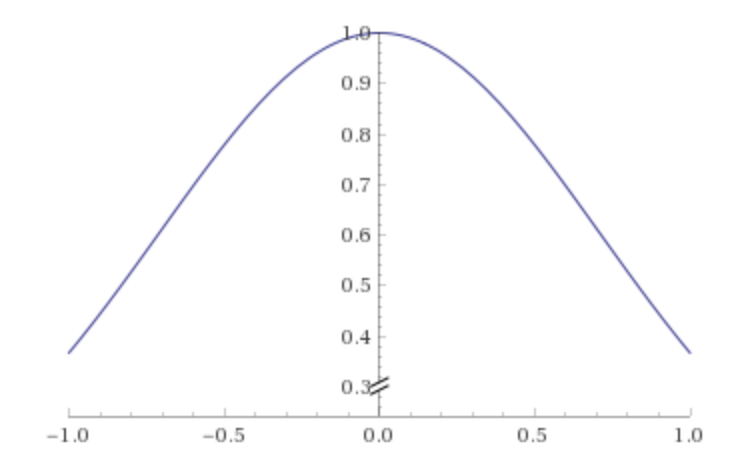
\includegraphics[width=8cm]{assets/gaus1}
    \caption{}
\end{figure}

Čím je $\beta$ parameter väčší tým je táto funkcia strmšia, čo znamená, že víťaz bude mať veľkú hodnotu aktivácie
ale vzdialenejšie neuróny ju budú mať takmer nulovú.
Pre $\beta = 30$ graf vyzerá nasledovne:

\begin{figure}[H]
    \centering
    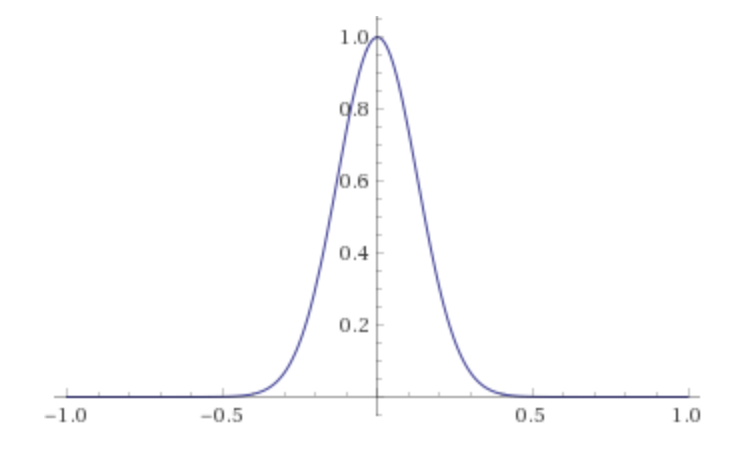
\includegraphics[width=8cm]{assets/gaus30}
    \caption{Leaky MSOM results}
\end{figure}

Samotnú hodnotu aktivácie sme chceli ešte normalizovať sumou všetkých aktivácii:
\begin{equation}
    y_{i} = \frac{\exp^{(-\beta \cdot d_{i}^{2})}}{\sum_{j} \exp^{(-\beta \cdot d_{j}^{2})}}
\end{equation}
Pri použití normalizácie sme dostávali signifikantne horšie výsledky
ako bez použitia normalizácie. Dôvodom bolo pravdepodobne to, že vychádzali veľmi malé
hodnoty aktivácií a rozdiely boli takmer veľmi malé. Z tohto dôvodu sme zostali 
pri pôvodnej nenormalizovanej verzii.

Hodnotu aktivácie určitého neurónu pri Activity RecSOM môžeme interpretovať aj nasledovne:
Aktivita neurónu vyjadruje bayesovskú pravdepdobnosť, že neurón bude víťazným neurónom.

\subsection{Activity RecSOM parametre}
V našom experimente sme vyskúšali kombinácie parametrov $\alpha$ a $\beta$.
Hodnoty parametra $\alpha$ sme zvolili z intervalu $<0, 1>$ s krokom $0.1$
Hodnoty parametra $\beta$ sme zvolili tak aby sme otestovali rôzne strmosti aktivačnej funkcie.
Konkrétne sme použili tieto hodnoty: $[5.0, 12.0, 13.0, 14.0, 15.0, 20.0, 30.0, 40.0, 50.0, 100.0]$
Pustili sme trénovanie na všetkých kombináciach parametrov $\alpha$ a $\beta$.

\subsection{Výsledky pre Activity RecSOM}

\begin{table}[h!]
    \centering
    \begin{tabular}{|c|c|} 
     \hline
     Parameter & Hodnota \\ 
     \hline\hline
     alpha & 0 - 1 (krok 0.1) \\ 
     \hline
     beta & [5.0, 12.0, 13.0, 14.0, 15.0, 20.0, 30.0, 40.0, 50.0, 100.0]\\ 
     \hline
     size & 30x30  \\
     \hline
     počet epôch & 10  \\
     \hline
     veľkosť posuvného okna & 15  \\
     \hline
    \end{tabular}
    \caption{Parametre Activity RecSOM siete}
    \label{table:1}
    \end{table}
    

\begin{figure}[H]
    \centering
    \begin{subfigure}{.5\textwidth}
        \centering
        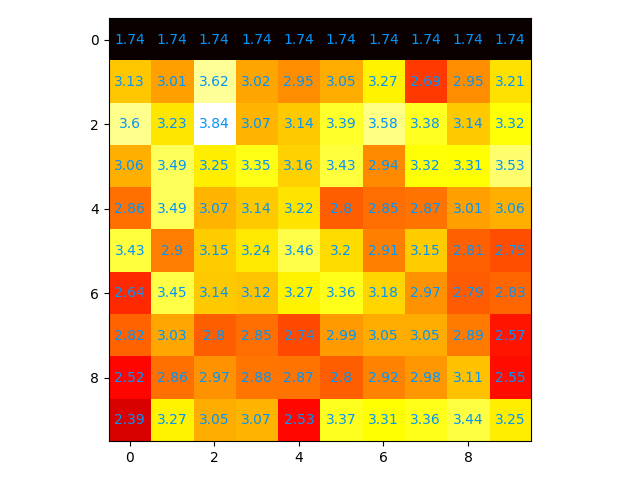
\includegraphics[width=\linewidth]{assets/activity_recsom_memory_span}
        \caption{Activity Recsom pamäťová hĺbka}
        \label{fig:sub1}
    \end{subfigure}%
    \begin{subfigure}{.5\textwidth}
        \centering
        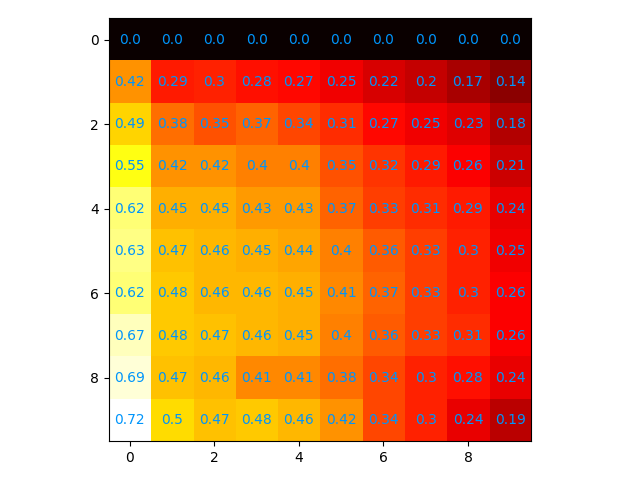
\includegraphics[width=\linewidth]{assets/activity_recsom_quantization_errors}
        \caption{Activity Recsom kvantizačná chyba}
        \label{fig:sub2}
    \end{subfigure}
    \caption{Heatmapy pre Activity RecSOM}
    \label{fig:test}
\end{figure}
    
\subsection{Analýza výsledkov Activity RecSOM}
Na x-ovej osy sú hodnoty parametra $\beta$ a na y-ovej osy sú hodnoty parametra $\alpha$.

Výsledky Activity RecSOM z hľadiska maximálnej hĺbky pamäte sú podobné výsledkom klasickej RecSOM a nie sú príliš 
zaujímavé. Keď je parameter $\alpha = 0$ je pamäťová hĺbka na minime, keďže kontext vtedy prakticky neexistuje.
Čo je však zaujimavé, je vplyv $\beta$ parametra na hodnoty pamäťovej hĺbky. Najvyššie hodnoty pamäťovej hĺbky sieť 
dosahuje pri vysokých hodnotách $\beta$ parametra $\beta > 20.0$. Čím vyššia je hodnota tohto parametra tým je aktivita
víťazného neurónu v kontexte viac odlíšená od aktivity ostatných neurónov (gausovská funkcia je strmšia), čo potvrdzuje naše predpoklady z 
experimentu s RecSOM sieťou. Príliš veľké množstvo nerelevantných informácii v kontexte má negatívny vplyv na pamäťovú hĺbku siete.
Čím viac sú vlastnosti kontextu sústredené na víťazný neurón, tým lepšie vyššie hodnoty pamäťovej hĺbky sieť dosahuje a naopak.

Na výsledkoch je vidno aj to, že čím má kontext vo výpočte vzdialenosti vyššiu váhu, tým sieť dosahuje horšie 
výsledky a tiež rastie aj kvantizačná chyba (sieť sa ťažšie učí), čo opäť potvrdzuje to, že príliš informačne bohatý kontext má negatívny vplyv
na pamäťovú hĺbku siete.

% ukazka testov s najlepsimi parametrami

\subsection{MSOM parametre}
Pri mSOM máme okrem $\alpha$ parametra, používaného pri výpočte vzdialenosti, opäť aj $\beta$ parameter, ktorý určuje váhu
váhového vektora víťaza z predchádzajúceho kroku $w_{i^{*}}$ a váhu kontextu
z predchádzajúceho kroku $y_{i^{*}}$ pri výpočte kontextu. Je nazývaný aj ako "zmiešavací" parameter
a určuje váhu jednotlivých zložiek vlastností víťazného neurónu v kontexte.
V našom experimente skúšame všetky kombinácie $\alpha$ a $\beta$ parametrov.
Hodnoty pre oba parametre sú z uzavretého intervalu $<0, 1>$ s krokom $0.1$ (100 experimentov).
Pri experimentovaní s mSOM sa snažíme zistiť aký vplyv má odlišný kontext, ktorý obsahuje iba informáciu
o víťazovi z predchádzajúceho kroku, na pamäťovú hĺbku siete. mSOM má veľkú výhodu v signifikantne 
vyššej rýchlosti učenia, vďaka zredukovanej dimenzie kontextu.

\subsection{Výsledky pre mSOM}

\begin{table}[h!]
    \centering
    \begin{tabular}{|c|c|} 
     \hline
     Parameter & Hodnota \\ 
     \hline\hline
     alpha & 0 - 1 (krok 0.1)  \\ 
     \hline
     beta & 0 - 1  (krok 0.1) \\ 
     \hline
     size & 30x30  \\
     \hline
     počet epôch & 10  \\
     \hline
     veľkosť posuvného okna & 15  \\
     \hline
    \end{tabular}
    \caption{Parametre mSOM siete}
    \label{table:1}
    \end{table}
    

\begin{figure}[H]
    \centering
    \begin{subfigure}{.5\textwidth}
        \centering
        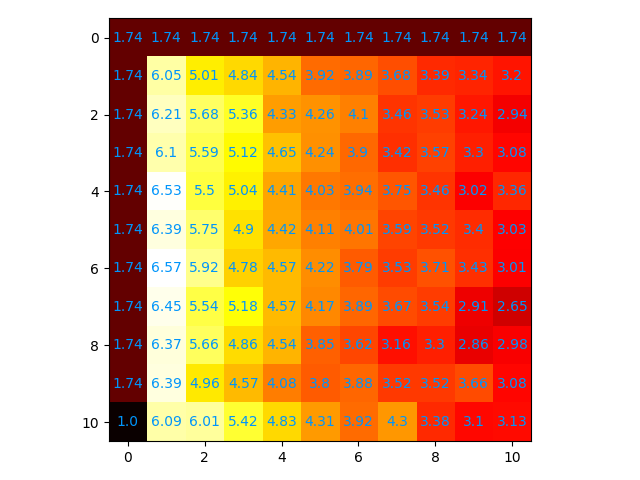
\includegraphics[width=\linewidth]{assets/msom_memory_span}
        \caption{mSOM pamäťová hĺbka}
        \label{fig:sub1}
    \end{subfigure}%
    \begin{subfigure}{.5\textwidth}
        \centering
        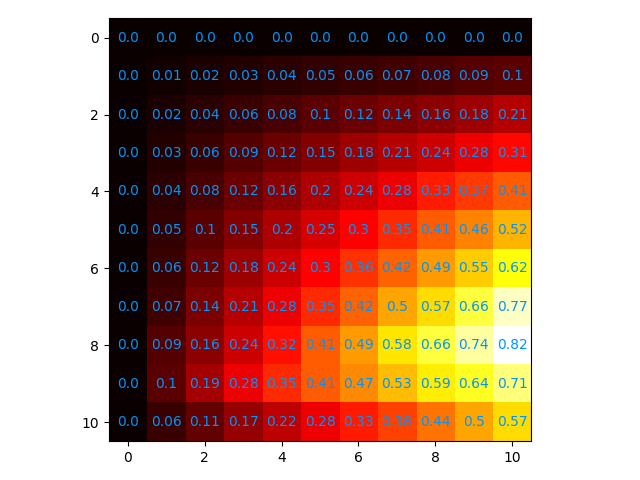
\includegraphics[width=\linewidth]{assets/msom_quantization_errors}
        \caption{mSOM kvantizačná chyba}
        \label{fig:sub2}
    \end{subfigure}
    \caption{Heatmapy pre mSOM}
    \label{fig:test}
\end{figure}
 Na x-ovej osy sú hodnoty parametra $\alpha$ a na y-ovej osy sú hodnoty parametra $\beta$. 
 Pamäťová hĺbka pri mSOM dosahuje minimá v ak je jeden z parametrov $\alpha$ alebo $\beta$ nulový a teda sieť nemá
 žiadny alebo len minimálny kontext. Ak je $\alpha = 0$, tak sa zanedbáva kontextová zložka pri výpočte vzdialenosti a 
 teda aj pri samotnom trénovaní siete a keď je $\beta = 0$ tak sa zanedbávajú váhy víťaza z predchádzajúceho kroku pri výpočte kontextu.
 Minimum pamäťovej hĺbky mSOM dosahuje ak sú $\alpha$ aj $\beta$ nulové.

 mSOM dosahuje najvyššie hodnoty pamäťovej hĺbky celkovo zo všetkých testovaných sietí, pričom je to zároveň 
 výpočtovo najefektívnejšia verzia rekurentnej SOM. 
 Maximálne hodnoty pamäťovej hĺbky dosahuje pri nízkych hodnotách $\alpha = 0.2 $, čo znamená že pri výpočte vzdialenosti má vyššiu váhu vzdialenosť vstupu od 
 váhového vektora ako vzdialenosť kontextu od kontextového vektora. 
 Pri maximách sú hodnoty parametra $\beta$ sú okolo hodnoty $0.5$, čo znamená, že obe zložky kontextu 
 (vlastnosti víťazného neurónu z predchádzajúceho kroku a samotný kontext z predchádzajceho kroku) sú rovnako dôležité.
 Pri maximách má sieť aj nízku kvantizačnú chybu a teda učí sa správne. 
 Najvyššie hodnoty kvantizačnej chyby sieť dosahuje ak sú oba parametre vysoké. Toto opäť potvrdzuje, že ak majú rekurentné
 siete príliš veľa informácii o kontexte a príliš málo informácii z aktuálneho vstupu, tak sa horšie trénujú.


 Čo je pri mSOM najzaujímavejšie je to, že nám tieto výsledky opäť potvrdili predpoklady, ktoré sme zistili pre recSOM a Activity recSOM a to že
 kontext nemusí obsahovať príliš veľa informácii. Pri mSOM kontext obsahuje iba kombináciu vlastností víťazného neurónu z predchádzajúceho kroku a teda tento 
 experiment s mSOM nám potvrdil, že pre pamäťovú hĺbku siete sú najdôležitejšie vlastnosti víťazného neurónu.

 mSOm dosiahla najlepšie výsledky spomedzi všetkých testovaných sietí.

% vyhodnotenie vysledkov experimentu

% ukazka testov s najlepsimi parametrami

\subsection{Decaying mSOM}
Pre potreby nášho experimentu sme si vytvorili ďaľšiu modifikovanú verziu % prida poznamku pod ciarou
rekurentnej SOM. Pri RecSOM kontext tvorí vektor aktivácii všetkých neurónov z predchádzajúceho kroku, 
pri mSOM je to kombinácia vlastností víťazného neurónu z predchádzajúceho kroku. 
Preto sme sa rozhodli použiť odlišný typ kontextu, ktorý bude tvorený kombináciou predchádzajúcih vstupov 
siete a nie stavmi siete z minulých krokov.
Zvyšné vlastnosti siete zostávajú rovnaké ako v iných rekurentných SOM.

Kontext počítame pomocou nasledujúceho rekurzívneho vzťahu:
\begin{equation}
	c = \beta^{0} \cdot x_{t} + \beta^{1} \cdot x_{t-1} + 
	\beta^{2} \cdot x_{t-2} \ddots \beta^{n} \cdot x_{t-n}
\end{equation}

$\beta$ parameter je číslo z intervalu $\beta < 1 \wedge \beta > 0$ a
$x_t, x_{t-1}, x_{t-2} ...$ sú vstupné vektory z predchádzajúcich krokov.
$t$ je číslo aktuálneho kroku a $n$ je veľkosť trénovacej množiny.

Z rekurzívneho vzťahu vyplýva, že kontext je tvorený kombináciou predchádzajúcich vstupov
pričom čím dávnejší je vstup, tým menšiu váhu má vo výslednom kontexte, čo je zabezpečené umocňovaním
$\beta$ parametra. Toto sa nazýva leaky integration. V našom prípade
to znamená, že dávne vstupy postupne strácajú na dôležitosti pričom sa stále sa podieľajú 
na vytváraní výsledného kontextu.

Čím je hodnota parametra $\beta$ vyššia, tým viac informácii z predchádzajúcich vstupov v sebe
kontext obsahuje. Dôležitosť dávnejších vstupov exponenciálne klesá.

\subsection{Decaying MSOM}
V experimente opäť skúšame všetky kombinácie $\alpha$ a $\beta$ parametrov.
Hodnoty pre oba parametre sú z uzavretého intervalu $<0, 1>$ s krokom $0.1$.

\subsection{Výsledky pre Decaying msom}
\begin{table}[h!]
    \centering
    \begin{tabular}{|c|c|} 
     \hline
     Parameter & Hodnota \\ 
     \hline\hline
     alpha & 0 - 1 (krok 0.1)  \\ 
     \hline
     beta & 0 - 1  (krok 0.1) \\ 
     \hline
     size & 30x30  \\
     \hline
     počet epôch & 10  \\
     \hline
     veľkosť posuvného okna & 15 \\
     \hline
    \end{tabular}
    \caption{Parametre RecSOM siete}
    \label{table:1}
    \end{table}
    
\begin{figure}[H]
    \centering
    \begin{subfigure}{.5\textwidth}
        \centering
        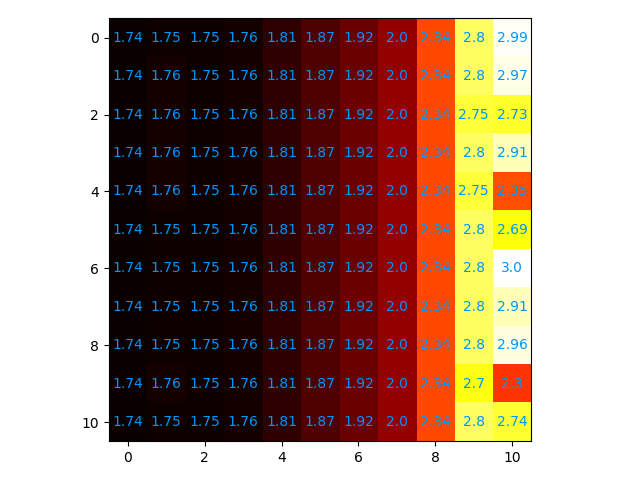
\includegraphics[width=\linewidth]{assets/decay_msom_memory_span}
        \caption{Decay mSOM pamäťová hĺbka}
        \label{fig:sub1}
    \end{subfigure}%
    \begin{subfigure}{.5\textwidth}
        \centering
        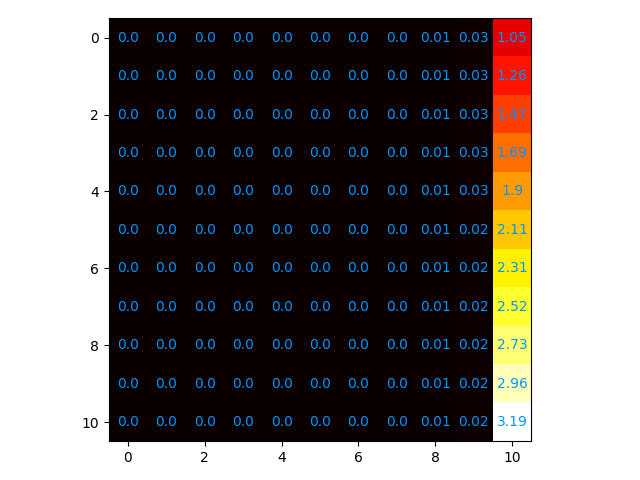
\includegraphics[width=\linewidth]{assets/decay_msom_quantization_errors}
        \caption{Decay mSOM kvantizačná chyba}
        \label{fig:sub2}
    \end{subfigure}
    \caption{Heatmapy pre Decay mSOM}
    \label{fig:test}
\end{figure}
    
Na x-ovej osy sú hodnoty parametra $\beta$ a na y-ovej osy sú hodnoty parametra $\alpha$.
Najvyššie dosiahnuté hodnoty pamäťovej hĺbky pri decay SOM sú porovnateľné s recSOM, resp. Activity recSOM.
Na grafe pamäťovej hĺbky je vidno, že hodnoty pamäťovej hĺbky závisia iba od hodnoty parametra $\beta$ v rekurzívnom vzťahu
pre výpočet kontextu.
Maximálne hodnoty pamäťovej hĺbky sieť dosahuje parameter $\beta = 1$. To znamená, že všetky predchádzajúce vstupy v kontexte majú
rovnakú váhu, avšak sieť sa pri takto bohatom kontexte minulých vstupov nedokáže dobre natrénovať, čo je vidno na grafe kvantizačných chýb.
Týmto experimentom sme vyskúšali aký vplyv na pamäťovú hĺbku siete má úplne odlišný druh kontextu a či sme s ním schopný sieť natrénovať.
Ukázalo sa, že s takýmto kontextom dokážeme dosiahnuť podobné výsledky ako s RecSOM. 
Pri RecSOM kontext obsahuje reprezentáciu vplyvov jednotlivých minulých vstupov na sieť a tu je to kombinácia samotných vstupov. 

% vyhodnotenie vysledkov experimentu

% ukazka testov s najlepsimi parametrami


Experimentami sme zistili, že na hĺbku pamäte siete má najväčší vplyv samotné zloženie kontextu.

Najdôležitejšie parameter, ktoré vplývajú na hĺbku pamäte neurónovej siete sú parameters $\alpha$ a $\beta$
vo vzťahu pre výpočet vzdialenosti vstupného vektora od určitého neurónu v siete (čiže od jeho váhového a kontextového vektora).
% TODO pridat rovnicu na ilustraciu
Tieto dva parameters určujú pomer dôležitosti aktuálneho vstupu a dôležitosť kontextu, pri výpočte vzdialenosti (kvantizačnej chyby).

Experiment prebiehal nasledujúcim spôsobom:
\begin{itemize}
    \item Vybrali sme vhodnú trénovaciu sekvenciu, počet epôch trénovania a dostatočnú veľkosť pamäťového okna
    \item Spustili sme trénovanie na všetkých kombináciach týchto dvoch parametrov s krokom 0.1
    \item Hodnoty pamäťovej hĺbky sme ukladali do súboru
    \item Na záver sme vykreslili heatmapu, ktorá znázorňuje aká bola pamäťová hĺbka pre rôzne kombinácie parametrov.
\end{itemize}

\section{Experiment so SRN a Reberovým automatom}
SRN má niektoré vlastnosti podobné so samoorganizujúcimi sa mapami. 
Na svojej skrytej vrstve si vytvára akokeby vysoko rozmernú somku. 

Naším hlavným cieľom pri experimente s SRN bolo preskúmať vlastnosti siete a pokúsiť sa nájsť 
spôsob merania a vyhodnotenia pamäťovej hĺbky.
SRN má tiež niekoľko zaujímavých vlastností, ktoré sme chceli preskúmať.

Experiment prebiehal nasledujúcim spôsobom:
Podobne ako pri experimentoch so samoorganizujúcimi sa mapami, ako prvé sme si potrebovali vytvorič vhodnú trénovaciu množinu.
Rozhodli sme sa, že použijeme rovnakú trénovaciu množinu ako pri samoorganizujúcich sa mapách.

Vstupom je vždy jedno písmeno zo sekvencie písmen $abcd$ a ako očakávaný výstup je vždy nasledujúce písmeno v sekvencii.
Takýmto spôsobom sme vytvorili trénovacie príklady.
Prvým krokom bolo overiť, či naša implementácia siete funguje správne. 
Ako chybovú funkciu sme použili log loss a aktivačnú funkciu na výstupnej vrstve sme použili softmax. 
Pri testovaní nám chyba klesala a sieť sa učila správne a predikovala korektné výsledky.

Keď sme mali funkčnú implementáciu SRN Elmanovej siete, natrénovali sme ju na vytvorenej trénovacej množine.

SRN si na kontextovej vrstve vytvára kontextovú reprezentáciu vstupov. Preto sme sa rozhodli, že 
správne natrénovanej SRN budeme postupne predkladať písmená z trénovacej množiny, pričom si po každej predikcii
, ktorú sieť spraví ukladáme kontextový vektor siete. 
Ku každému takémuto vektoru priradíme posuvné okno daného znaku z trénovacej množiny (podobne ako pri experimentoch so SOMkami).
Po predložení všetkých znakov z trénovacej množiny sieti sme dostali slovník posuvných okien a prislúchajúcimi kontextovými vektormi
zo siete.
Tieto dáta sme potrebovali nejakým spôsobom vizualizovať, aby sme videli nejaké súvislosti medzi reprezentáciou vstupov na kontextovej vrstve a 
podobnosťou samotných vstupov, na čo je vhodné použiť reprezentáciu vo forme dendogramu.
Na vykreslenie dendogramu je potrebné vytvoriť tzv. podobnostnú maticu (ang. similarity matrix), kde 
riadky aj stĺpce reprezentujú jednotlivé kontextové vektory a hodnoty v samotnej matici sú euklidovské vzdialenosti medzi týmito vektormi.
Z toho vyplýva, že na diagonále máme samé nulové hodnoty (rovnaké vektory majú nulovú vzdialenosť od seba).

% pridat ukazku similarity matrix

Z takejto matice potom vieme vytvoriť dendogram, ktorý znázorňuje súvislosti medzi euklidovskou vzdialenosťou jednotlivýh vektorov a samotnými posuvnými oknami z trénovacej množiny.
Z toho vieme potom povedať, ktoré vstupy sú vo vnútornej reprezentácii SRN blízke. 




Zaujímavou vlastnosťou SRN je aj to, že si na skrytej vrstve dokáže vytvoriť vlastnú reprezentáciu stavového automatu, ak 
je trénovaná na trénovacej množine, ktorá je tvorená stringom generovaným reberovým automatom. Vďaka tejto vlastnosti
by sa mala SRN natrénovať na takejto trénovacej množine s nulovou chybou.



Pri SRN sme opäť použili vlastnú modifikovanú implementáciu siete, aby sme boli schopní
ukladať si kontext siete pri predikovaní.






